\begin{figure}[h!]
    \centering
    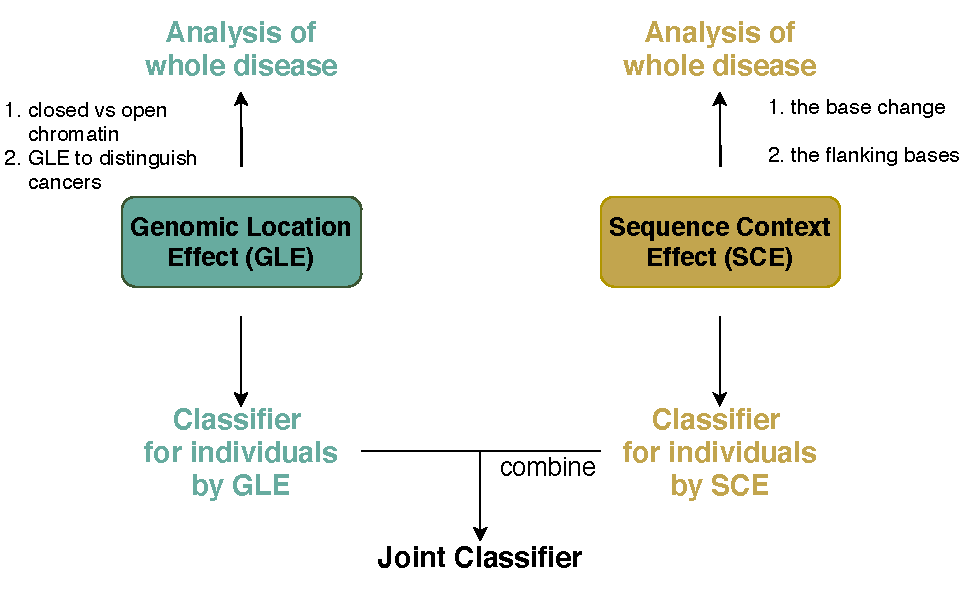
\includegraphics[scale=0.85]{graphics/workflow.pdf}
    \caption{\textbf{Project workflow for understanding cancer mutagenesis data and exploiting it for cancer classification.} On one hand, cancers were analysed on the whole disease scale, which considered mutations from all donors of the same diseases as a whole. This magnified the signals in the data and made it easier for understanding the mutagenesis process. On the other hand, the information from the factors analysed above was used for training a classifier on the individual donor scale, meaning that this classifier could potentially be applied to a new patient's mutation data to predict their cancer. This followed a standard machine learning training procedure, outlined in Section \ref{methods:ml}.}
    \label{fig:workflow}
\end{figure}
